%%%%%%%%%%%%%%%%%%%%%%%%%%%%%%%%%%%%%%%%%%%%%%%%%%%%%%%%%%%%%%%%%%%%%%%%%%%%%%%%%%
\begin{frame}[fragile]\frametitle{}
\begin{center}
{\Large Introduction to LangChain}
\end{center}
\end{frame}

%%%%%%%%%%%%%%%%%%%%%%%%%%%%%%%%%%%%%%%%%%%%%%%%%%%%%%%%%%%%%%%%%%%%%%%%%%%%%%%%%%
\begin{frame}\frametitle{What is LangChain?}

\begin{itemize}
\item LangChain can be used to work with Large Language Models (LLMs). 
\item To answer questions about a specific field, like medicine or law. 
\item Popular framework for fine tuning with custom corpus.
\end{itemize}

\begin{center}
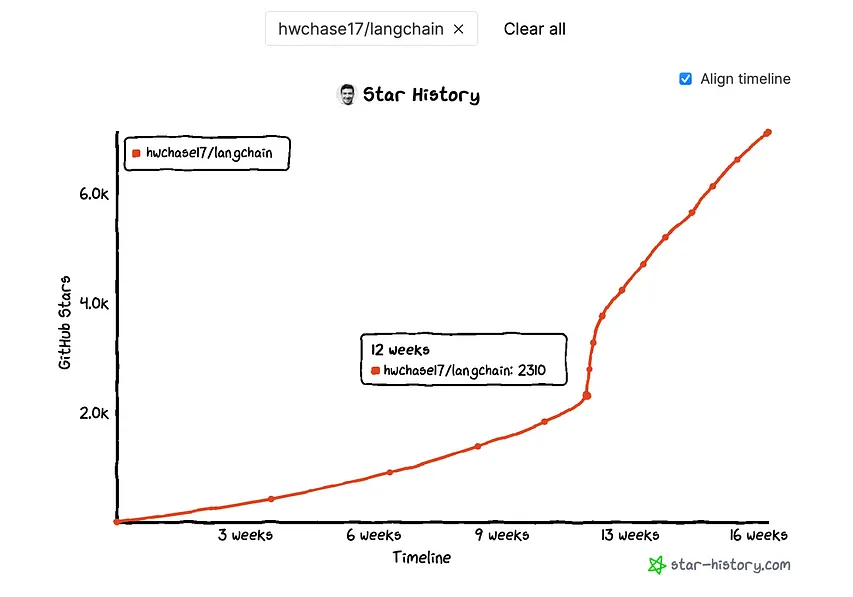
\includegraphics[width=0.6\linewidth,keepaspectratio]{langchain3}
\end{center}	  


{\tiny (Ref: Getting started with LangChain - Avra)}
\end{frame}

%%%%%%%%%%%%%%%%%%%%%%%%%%%%%%%%%%%%%%%%%%%%%%%%%%%%%%%%%%%%%%%%%%%%%%%%%%%%%%%%%%
\begin{frame}\frametitle{How LangChain Works?}

\begin{itemize}
\item Text is preprocessed by breaking it down into chunks or summaries, 
\item embedding them in a vector space, 
\item searching for similar chunks when a question is asked. 
\end{itemize}

\begin{center}
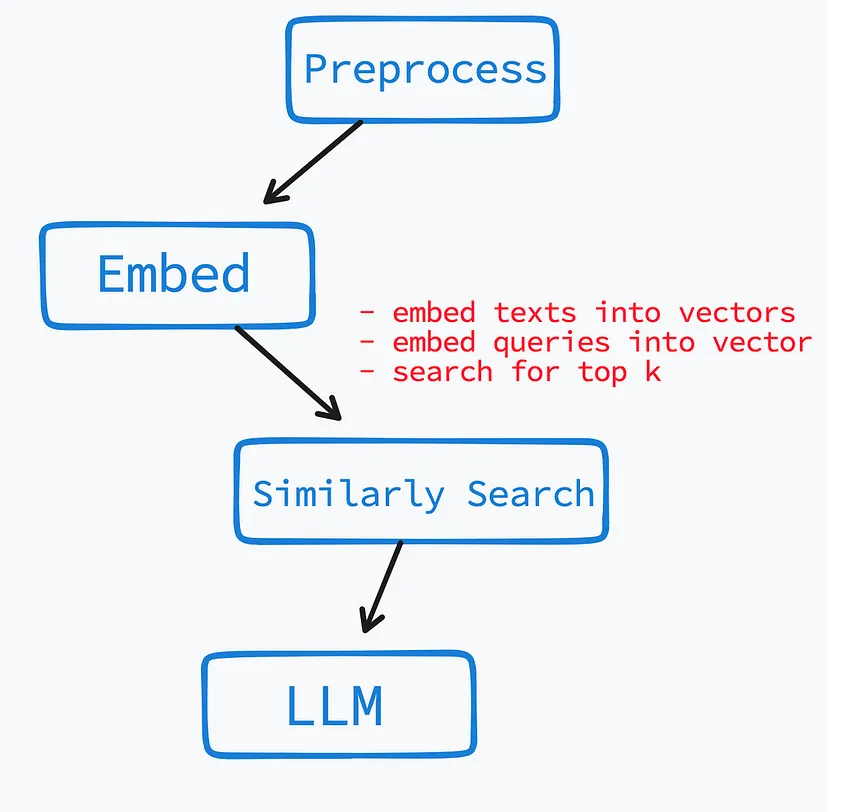
\includegraphics[width=0.5\linewidth,keepaspectratio]{langchain4}
\end{center}	  


{\tiny (Ref: Getting started with LangChain - Avra)}
\end{frame}


%%%%%%%%%%%%%%%%%%%%%%%%%%%%%%%%%%%%%%%%%%%%%%%%%%%%%%%%%%%%%%%%%%%%%%%%%%%%%%%%%%
\begin{frame}\frametitle{LangChain Components}

\begin{center}
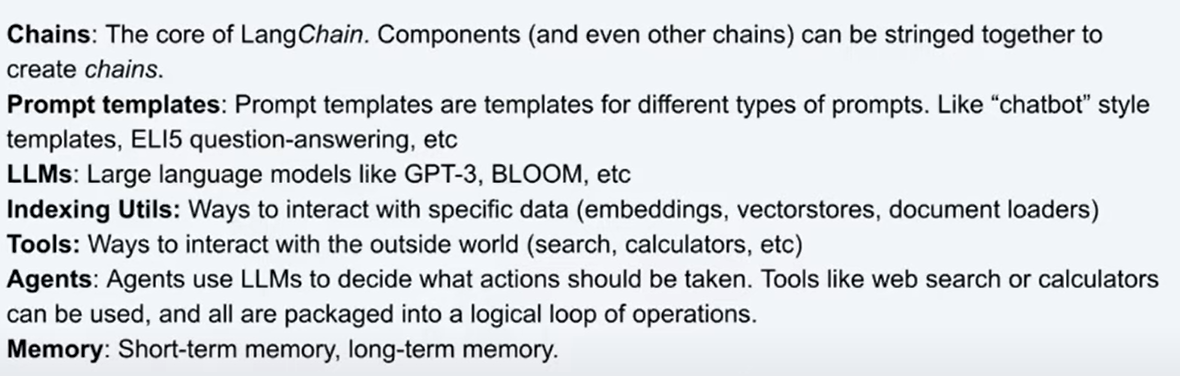
\includegraphics[width=\linewidth,keepaspectratio]{langchain1}
\end{center}	  

{\tiny (Ref: Building the Future with LLMs, LangChain, \& Pinecone)}
\end{frame}

%%%%%%%%%%%%%%%%%%%%%%%%%%%%%%%%%%%%%%%%%%%%%%%%%%%%%%%%%%%%%%%%%%%%%%%%%%%%%%%%%%
\begin{frame}\frametitle{Chains}

\begin{itemize}
\item Enable users to combine multiple components together to create a single, coherent application.
\item Example: takes user input, formats it using a PromptTemplate, and then passes the formatted response to a Large Language Model (LLM) for processing.
\item Sequential chains: output of the first LLM becomes the input to the second LLM and so on
\end{itemize}

\begin{center}
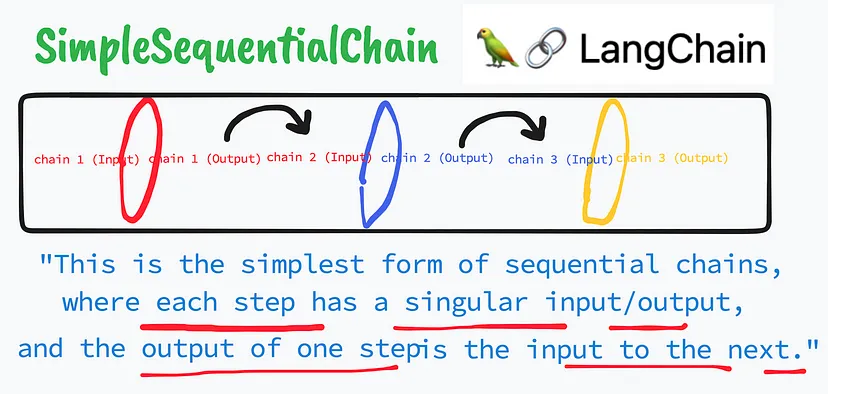
\includegraphics[width=0.8\linewidth,keepaspectratio]{langchain5}
\end{center}	  


{\tiny (Ref: Getting started with LangChain - Avra)}
\end{frame}

%%%%%%%%%%%%%%%%%%%%%%%%%%%%%%%%%%%%%%%%%%%%%%%%%%%%%%%%%%%%%%%%%%%%%%%%%%%%%%%%%%
\begin{frame}[fragile] \frametitle{Chains}

{\tiny (Ref: Getting started with LangChain - Avra)}


\begin{lstlisting}
    # Chain 1: Generating a rephrased version of the user's question
    template = """{question}\n\n"""
    prompt_template = PromptTemplate(input_variables=["question"], template=template)
    question_chain = LLMChain(llm=llm, prompt=prompt_template)

    # Chain 2: Generating assumptions made in the statement
    template = """Here is a statement:
        {statement}
        Make a bullet point list of the assumptions you made when producing the above statement.\n\n"""
    prompt_template = PromptTemplate(input_variables=["statement"], template=template)
    assumptions_chain = LLMChain(llm=llm, prompt=prompt_template)
    assumptions_chain_seq = SimpleSequentialChain(
        chains=[question_chain, assumptions_chain], verbose=True
    )

\end{lstlisting}

\end{frame}

%%%%%%%%%%%%%%%%%%%%%%%%%%%%%%%%%%%%%%%%%%%%%%%%%%%%%%%%%%%%%%%%%%%%%%%%%%%%%%%%%%
\begin{frame}[fragile] \frametitle{Chains}

{\tiny (Ref: Getting started with LangChain - Avra)}


\begin{lstlisting}
    # Chain 3: Fact checking the assumptions
    template = """Here is a bullet point list of assertions:
    {assertions}
    For each assertion, determine whether it is true or false. If it is false, explain why.\n\n"""
    prompt_template = PromptTemplate(input_variables=["assertions"], template=template)
    fact_checker_chain = LLMChain(llm=llm, prompt=prompt_template)
    fact_checker_chain_seq = SimpleSequentialChain(
        chains=[question_chain, assumptions_chain, fact_checker_chain], verbose=True)
    # Final Chain: Generating the final answer to the user's question based on the facts and assumptions
    template = """In light of the above facts, how would you answer the question '{}'""".format(user_question)
    template = """{facts}\n""" + template
    prompt_template = PromptTemplate(input_variables=["facts"], template=template)
    answer_chain = LLMChain(llm=llm, prompt=prompt_template)
    overall_chain = SimpleSequentialChain(
        chains=[question_chain, assumptions_chain, fact_checker_chain, answer_chain],
        verbose=True,)
\end{lstlisting}


\end{frame}

%%%%%%%%%%%%%%%%%%%%%%%%%%%%%%%%%%%%%%%%%%%%%%%%%%%%%%%%%%%%%%%%%%%%%%%%%%%%%%%%%%
\begin{frame}\frametitle{Chains}

The SimpleSequentialChain combines several chains of operations to run a pipeline. 

\begin{itemize}
\item question\_chain: This chain takes the user's question as input and returns it as output. 
\item assumptions\_chain: This chain takes the output from question\_chain as input and produces a bullet-point list of assumptions based on a statement related to the question. 
\item fact\_checker\_chain: This chain takes the outputs from question\_chain and assumptions\_chain as inputs and produces a bullet-point list of assertions based on the question and assumptions.
\item answer\_chain: This chain takes the outputs from question\_chain, assumptions\_chain, and fact\_checker\_chain as inputs and produces an answer to the user's question based on the facts generated by the previous chains.
\end{itemize}


{\tiny (Ref: Getting started with LangChain - Avra)}
\end{frame}


%%%%%%%%%%%%%%%%%%%%%%%%%%%%%%%%%%%%%%%%%%%%%%%%%%%%%%%%%%%%%%%%%%%%%%%%%%%%%%%%%%
\begin{frame}\frametitle{Prompt Engineering}

\begin{center}
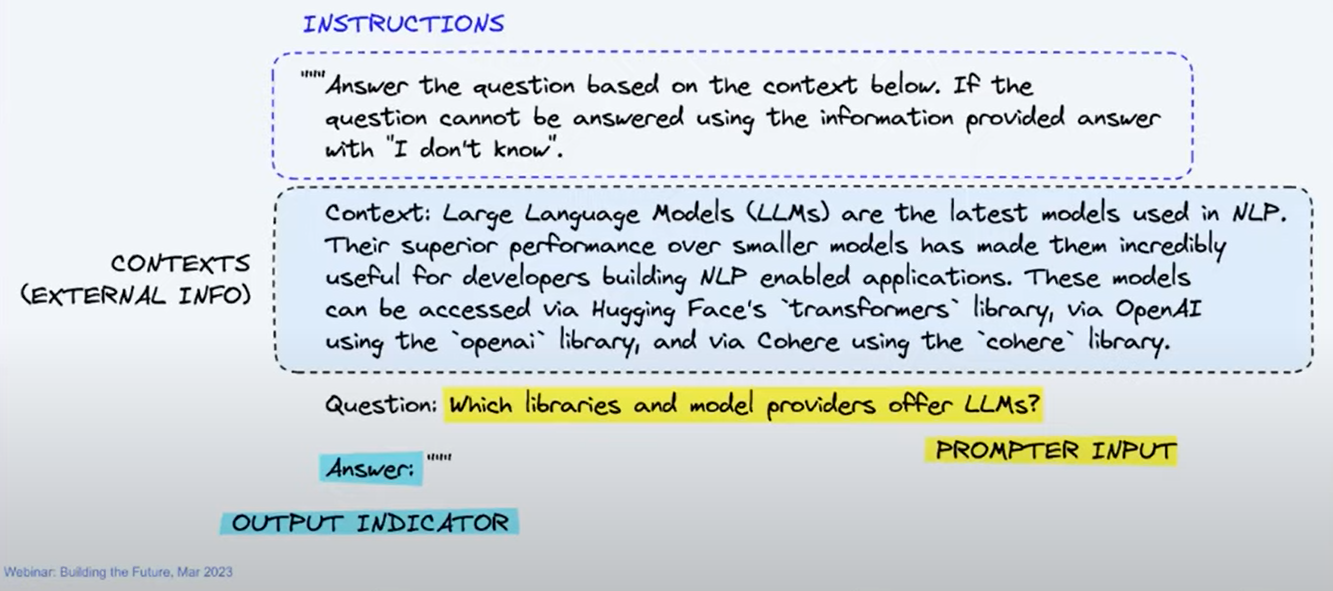
\includegraphics[width=\linewidth,keepaspectratio]{langchain2}
\end{center}	  

{\tiny (Ref: Building the Future with LLMs, LangChain, \& Pinecone)}
\end{frame}